	\section{Introduction}
%
%1. Context
%2. Problem
%3. Problem relevant and nontrivial
%4. Not solved before
%5. My Plan for solving it

``To move at full speed, it’s crucial to bring the networking operations teams into the DevOps chain,...''\footnote{https://siliconangle.com/2019/02/19/cloud-native-networking-for-devops-leaves-sdn-in-the-dust-cubeconversations-startupoftheweek/}.

Many advances have been made in recent years towards making applications ready for the special environment of the cloud. Development of such programs needs to be adapted in order to be effective and efficient since it significantly departs from previous settings. Matthew Foemmel and Martin Fowler have proposed the influential practice of Continuous Integration and Deployment \cite{fowler_2006} \cite{fowler_foemmel_2000} in order to tackle the development side of this complex process. In their original work from 2000 they base their approach  on four principles:
\begin{enumerate}
	\item Single place for the source code
	\item Automated build process
	\item Automated tests
	\item Make executable reachable
\end{enumerate}
This process provides a solid basis for the collaboration on any software project, but is especially useful when working on a project that has its place in the cloud. 

This paradigm has been expanded to not only comprise the development part, but also architectural best practices in the so-called 12-factor methodology as formulated by Adam Wiggins. and drafted by employees of the cloud platform Heroku.  It summarizes the most important aspects that need to be taken into consideration to make life easier when designing cloud native applications. These guidelines contain strategies to avoid recurring problems when developing in the cloud environment, like the fragmentation of the codebase, keeping track of and managing all needed dependencies, placing the configuration in the environment and many more \cite{hofmann2017microservices} \cite{12Factor}. 

While there have been many advances in making applications ready for the cloud  and using automated build chains like in Continuous Integration and Delivery,  the networking infrastructure has long remained old-school monolithic. Functionalities that are specific to the setup, orchestration, administration and enhancement of large scale networks have long been implemented into specialized hardware middleboxes. Such services range from the security domain (intrusion detection, firewalls) to the optimization of the Wide Area Network (WAN). Deploying and managing dedicated hardware for such services quickly results in high investment and operation costs and hugely limits the flexibility of the network. With the ever growing reliance on cloud networks and infrastructures to provide a plethora of services, it is crucial that the management of the underlying network is made much more reactive and adaptable. 

In order to take full advantage of the highly modular and flexible cloud concepts, the supporting network has to be able to quickly and reliably adapt to changes. The guiding question for this paper is to give an overview and evaluate concepts that have been put forward to tackle these limitations by applying the previously mentioned strategies to the network domain.

A first step into this direction can be taken by providing network functions  and services that have traditionally been dependent on proprietary and custom hardware as virtualized and independent software entities that can run on general-purpose hardware. This should break up the dependency on specialized middleboxes, and facilitate the provisioning and management of the services. Although virtualization has had a great impact, there still are unsolved problems that need addressing. These include and are not limited to the speed of upgrades and restarts, limited scalability and the fact that often services have been ported to the cloud in a \textit{lift and shift manner} without taking full advantage of the Cloud paradigm \cite{CNF}.

In a second step it is important to find solutions to these problems, especially when thinking about how it is possible to efficiently design and manage virtualized network functions. Orienting these functions along the lines of the cloud has coined the term of \textit{Cloud Native Network Functions} \cite{CNF} \cite{inproceedings} \cite{evolutionnfv}. 



\section{Related Work}
This section is about work that is related to the topic of my seminar thesis, you know?

\section{Enabling Technologies}
Extending Networking into the Virtualization Layer (see \cite{pfaff2009extending}) summarizes how the traditionally monolithic and physically bound domain of networking can be broken up and modularized by means of virtualization. The following three parts would focus on enabling and supporting technologies needed to realize the vision of this new paradigm. First, the business logic needs to be packaged and executed. This can happen in virtual machines, containers etc. Following that, virtualized switching technology needs to be put in place to allow for successful packet forwarding. One technology is Open vSwitch which is an implementation of a virtual switch, connecting virtual interfaces of VMs for instance with physical interfaces. Docker and Kubernetes additionally provide means for communication between several, executable artifacts.
\todo{You quickly move to a tool/implementation. Can you stay on the conceptual level more before you dive into possible solutions? Maybe explain that using a diagram would help?} 
\subsection{Virtual Machines to Containerization}
\subsection{Open vSwitch}
\subsection{Kubernetes as Container orchestrator}

\quad

\section{Network Functions}
Before venturing into Virtualized Network Functions, it needs to be clarified what network functions are in general, how they are implemented and composed \textit{physically}, and what the motivations are to move towards virtualizing them. 
\subsection{Physical Network Service Composition}
The inner makings of a cloud: A lot of custom hardware (middleboxes) for services like intrusion detection, firewalls and the optimization of the Wide Area Network (WAN) have often been used (and still used to this day), in extremely high numbers. This leads to several impairments with growing networks: High investment costs, high operational costs, no or limited upgradeability and automatization   \cite{sherry2016middleboxes}. This part shall provide motivation to use aforementioned technologies to provide a more flexible and automatable solution. This will only gain importance with higher complexity and higher demand of the networks that are being built (Growing cloud data centers, implementation of 5G, etc). 

\subsection{Network Virtualization}
\subsubsection{Software Defined Networking}
\begin{description}
	\item [SDN] SDN: Breakup of the control and data plane, routing hardware (switches) can be organized and ()re-)configured from a distributed controller software without the need of cumbersome manual efforts.
\end{description}

\subsubsection{Virtualized Network Functions in Network Function Virtualization ( VNFs vs NFVs )}
NFV and VNF basics \cite{mijumbi2016network} NFV real-world impact \cite{bilal2016impact} Service orchestration \cite{de2018network}

\begin{description}
	\item [VNF] Can complement the SDN paradigm (but can exist independently)  by providing functionality needed in the network domain as an executable artifact
	\item [NFV] NFV integrates VNFs into a system that can manage and deploy these functions in sensible manner. 
\end{description}
\todo{References for the definitions}
\subsubsection{Organizations and Motivations}
ETSI proposing NFV architecture already in 2012 in a white paper  \cite{nfv_wp}. The CNCF (Cloud-native Computing Foundation) has launched a testbed to compare the performance of VNFs on an OpenStack enviromnent versus a Kubernetes setup \footnote{https://www.cncf.io/announcement/2019/02/25/cncf-launches-cloud-native-network-functions-cnf-testbed/}	

\section{Cloud-native NFV}

\begin{figure}
	\centering
	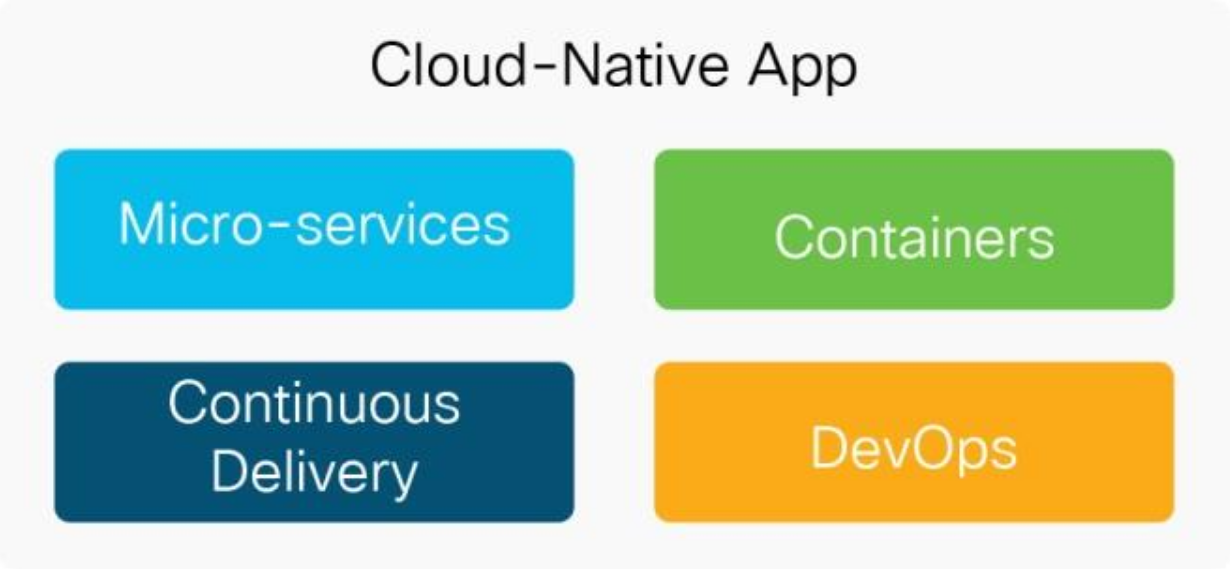
\includegraphics[width=0.75\linewidth]{images/cloudNativeApp.png}
	\caption{This is the caption \cite{CNF}}
	\label{img:cloudNativeApp}
\end{figure}

\subsection{Interoperability of VNFs}
A lot of proprietary and custom build environments which VNFs are build for and deployed onto. This limits their effectiveness considerably.
\subsection{Design Principles for Cloud-native VNFs }
What is cloud-native, how do these principles relate to  the networking domain? Whitepapers published by Analysys Mason \cite{evolutionnfv} and Cisco \cite{CNF}
\subsection{Managing VNFs efficiently (CI/CD and Management)}
Virtual Machines, Openstack vs Docker and Kubernetes managing and orchestrating the deployment of network functionality, what are the benefits? What are drawbacks?
\subsection{Cloud-native network functions}
Definition, advantages, state-of-the-art, testbed 
\todo{I am missing somewhat talking about the problems. What are the challenges that NF solve in general? What changes in the cloud native / K8s world? What does that mean for the challenges that traditional NF solve? I have the feeling, you jump too quickly to the solutions and showing advantages and disadvantages (which is great), but forget to define the problems and challenges clearly before. }

\section{Conclusion \& Future Work}
Combining several concepts like for instance an SDN-controller deploying and managing VNFs/CNFs  on demand could create even more efficient and interesting possibilities where specific functions and services could deploy dynamically when they are being requested. Lifecycle management can be done by the SDN-Controller. 
\todo{Future Work typically means what YOU would do if you had infinite time for your research. Not what the technology will be in the future. Try to use a different name for that section. Or did I read that wrongly?}


\section{List of references}
\begin{description}[style=sameline, leftmargin=1em, font=\normalfont]
	\item[Pfaff \cite{pfaff2009extending}]  Virtualization in Networking. Basics of how virtualization started to make its way into the networking domain. Overview of network architectures and topologies that employ virtualization. The starting of how to break up monoplithic network infrastructure with virtualization. The components decsribed here are the basis for VNFs (and the overarching NFV). 
	
	\item[Sherry \cite{sherry2016middleboxes}] Middleboxes as a Cloud Service. Traditional Network Functions are provided by specialized and proprietary middleboxes. What is their significance in 2016's enterprise and educational networks? The results of this paper motivate towards decoupling functionality from physical boxes and providing virtualized solutions.
	
	\item [Mijumbi \cite{mijumbi2016network}] NFV State of the art . Comprehensive overview of the state of the art of NFVs with focus on Telephony Service Providers. Interesting because critical evaluation of NFV solutions that, contrary to their original design, seem to result in a means to pool vendor specific resources together instead of supporting real interoperability. 
	
	\item [Bilal \cite{bilal2016impact}] Impact of CNFs . The authors analyze resource consumption of a real-life example, namely two different mobile networks and evaluate the impact virtualization would have on these networks. 
	
	\item [De Sousa \cite{de2018network}] Network Service Orchestration. The Network Service Orchestration is in the focus of this paper. The authors lay out a comprehensive survey over service orchestration technologies and additionally provide a taxonomy.  
	
	\item[NFV White Paper \cite{nfv_wp}]  The white paper lays out the foundation for NFV. 
	
	\item [AM White Paper \cite{evolutionnfv}] This white paper, seemingly sponsored by  Huawei, focuses on CNFs for telecommunication companies, including migration strategies from NFV to CNFs. 
	
	\item [CNF White Paper by Cisco \cite{CNF}] A white paper sponsored by Cisco provides insights into the point-of-view of a vendor. They set out to define what CNFs are, and how potential clients can benefit from them. They use Kubernetes as the main orchestrator and suggest it for further roles, too. 
	
	\item [Cloud-native 5G \cite{inproceedings}] The authors layout the implementation of VNFs that adhere to Cloud-native design principles for 5G. Furthermore they summarize existing projects and show an exemplary Use Case for this technology. Very relevant to my work, they use Docker for prototyping and are migrating to Kubernetes for the Cloud Native NFVI (Network Functions Virtualization Infrastructure) interface. 
	
	\todo{5G would also bring in an interesting perspective. You could show what kind of challenges are introduced with 5G for the network as well. }
	\todo{Reference/Specification for NFVI}
	
\end{description}